\begin{figure}[!h]
	\centering
	\subbottom[an example building\label{fig:egorgimg}]{
		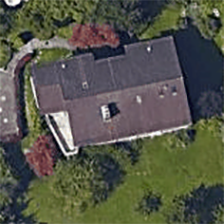
\includegraphics[width=\figfigfig\textwidth]{2-01-0.png}
	}
	\subbottom[pixel-wise mask\label{fig:egpxlmsk}]{
		\frame{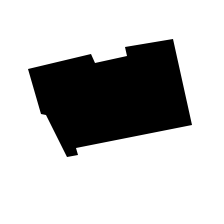
\includegraphics[width=\figfigfig\textwidth]{2-01-1.png}}
	}
	\subbottom[polygon prediction\label{fig:egpoly}]{
		\frame{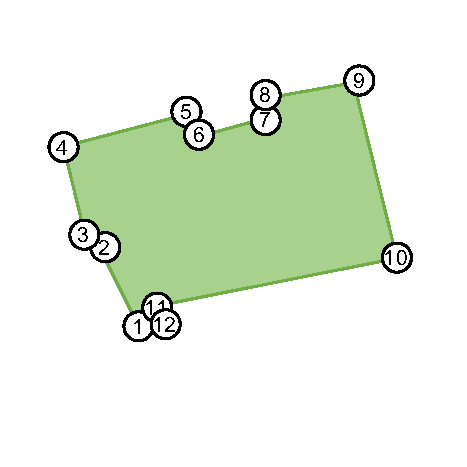
\includegraphics[width=\figfigfig\textwidth]{2-01-2.pdf}}
	}
    \caption[Comparison of pixel-wise mask and polygon]{Comparison of pixel-wise mask and polygon. (a) is the original image containing a building. (b) is the target mask of traditional pixel-wise instance segmentation, (c) is the desired prediction of polygon, of which the vertices are numbered.}
	\label{fig:egcmp}
\end{figure}